\documentclass[]{article}
\usepackage{lmodern}
\usepackage{amssymb,amsmath}
\usepackage{ifxetex,ifluatex}
\usepackage{fixltx2e} % provides \textsubscript
\ifnum 0\ifxetex 1\fi\ifluatex 1\fi=0 % if pdftex
  \usepackage[T1]{fontenc}
  \usepackage[utf8]{inputenc}
\else % if luatex or xelatex
  \ifxetex
    \usepackage{mathspec}
  \else
    \usepackage{fontspec}
  \fi
  \defaultfontfeatures{Ligatures=TeX,Scale=MatchLowercase}
\fi
% use upquote if available, for straight quotes in verbatim environments
\IfFileExists{upquote.sty}{\usepackage{upquote}}{}
% use microtype if available
\IfFileExists{microtype.sty}{%
\usepackage[]{microtype}
\UseMicrotypeSet[protrusion]{basicmath} % disable protrusion for tt fonts
}{}
\PassOptionsToPackage{hyphens}{url} % url is loaded by hyperref
\usepackage[unicode=true]{hyperref}
\hypersetup{
            pdftitle={Improvements to the dvir Package},
            pdfauthor={Alexander van der Voorn},
            pdfborder={0 0 0},
            breaklinks=true}
\urlstyle{same}  % don't use monospace font for urls
\usepackage[margin=1in]{geometry}
\usepackage{color}
\usepackage{fancyvrb}
\newcommand{\VerbBar}{|}
\newcommand{\VERB}{\Verb[commandchars=\\\{\}]}
\DefineVerbatimEnvironment{Highlighting}{Verbatim}{commandchars=\\\{\}}
% Add ',fontsize=\small' for more characters per line
\usepackage{framed}
\definecolor{shadecolor}{RGB}{248,248,248}
\newenvironment{Shaded}{\begin{snugshade}}{\end{snugshade}}
\newcommand{\KeywordTok}[1]{\textcolor[rgb]{0.13,0.29,0.53}{\textbf{#1}}}
\newcommand{\DataTypeTok}[1]{\textcolor[rgb]{0.13,0.29,0.53}{#1}}
\newcommand{\DecValTok}[1]{\textcolor[rgb]{0.00,0.00,0.81}{#1}}
\newcommand{\BaseNTok}[1]{\textcolor[rgb]{0.00,0.00,0.81}{#1}}
\newcommand{\FloatTok}[1]{\textcolor[rgb]{0.00,0.00,0.81}{#1}}
\newcommand{\ConstantTok}[1]{\textcolor[rgb]{0.00,0.00,0.00}{#1}}
\newcommand{\CharTok}[1]{\textcolor[rgb]{0.31,0.60,0.02}{#1}}
\newcommand{\SpecialCharTok}[1]{\textcolor[rgb]{0.00,0.00,0.00}{#1}}
\newcommand{\StringTok}[1]{\textcolor[rgb]{0.31,0.60,0.02}{#1}}
\newcommand{\VerbatimStringTok}[1]{\textcolor[rgb]{0.31,0.60,0.02}{#1}}
\newcommand{\SpecialStringTok}[1]{\textcolor[rgb]{0.31,0.60,0.02}{#1}}
\newcommand{\ImportTok}[1]{#1}
\newcommand{\CommentTok}[1]{\textcolor[rgb]{0.56,0.35,0.01}{\textit{#1}}}
\newcommand{\DocumentationTok}[1]{\textcolor[rgb]{0.56,0.35,0.01}{\textbf{\textit{#1}}}}
\newcommand{\AnnotationTok}[1]{\textcolor[rgb]{0.56,0.35,0.01}{\textbf{\textit{#1}}}}
\newcommand{\CommentVarTok}[1]{\textcolor[rgb]{0.56,0.35,0.01}{\textbf{\textit{#1}}}}
\newcommand{\OtherTok}[1]{\textcolor[rgb]{0.56,0.35,0.01}{#1}}
\newcommand{\FunctionTok}[1]{\textcolor[rgb]{0.00,0.00,0.00}{#1}}
\newcommand{\VariableTok}[1]{\textcolor[rgb]{0.00,0.00,0.00}{#1}}
\newcommand{\ControlFlowTok}[1]{\textcolor[rgb]{0.13,0.29,0.53}{\textbf{#1}}}
\newcommand{\OperatorTok}[1]{\textcolor[rgb]{0.81,0.36,0.00}{\textbf{#1}}}
\newcommand{\BuiltInTok}[1]{#1}
\newcommand{\ExtensionTok}[1]{#1}
\newcommand{\PreprocessorTok}[1]{\textcolor[rgb]{0.56,0.35,0.01}{\textit{#1}}}
\newcommand{\AttributeTok}[1]{\textcolor[rgb]{0.77,0.63,0.00}{#1}}
\newcommand{\RegionMarkerTok}[1]{#1}
\newcommand{\InformationTok}[1]{\textcolor[rgb]{0.56,0.35,0.01}{\textbf{\textit{#1}}}}
\newcommand{\WarningTok}[1]{\textcolor[rgb]{0.56,0.35,0.01}{\textbf{\textit{#1}}}}
\newcommand{\AlertTok}[1]{\textcolor[rgb]{0.94,0.16,0.16}{#1}}
\newcommand{\ErrorTok}[1]{\textcolor[rgb]{0.64,0.00,0.00}{\textbf{#1}}}
\newcommand{\NormalTok}[1]{#1}
\usepackage{longtable,booktabs}
% Fix footnotes in tables (requires footnote package)
\IfFileExists{footnote.sty}{\usepackage{footnote}\makesavenoteenv{long table}}{}
\usepackage{graphicx,grffile}
\makeatletter
\def\maxwidth{\ifdim\Gin@nat@width>\linewidth\linewidth\else\Gin@nat@width\fi}
\def\maxheight{\ifdim\Gin@nat@height>\textheight\textheight\else\Gin@nat@height\fi}
\makeatother
% Scale images if necessary, so that they will not overflow the page
% margins by default, and it is still possible to overwrite the defaults
% using explicit options in \includegraphics[width, height, ...]{}
\setkeys{Gin}{width=\maxwidth,height=\maxheight,keepaspectratio}
\IfFileExists{parskip.sty}{%
\usepackage{parskip}
}{% else
\setlength{\parindent}{0pt}
\setlength{\parskip}{6pt plus 2pt minus 1pt}
}
\setlength{\emergencystretch}{3em}  % prevent overfull lines
\providecommand{\tightlist}{%
  \setlength{\itemsep}{0pt}\setlength{\parskip}{0pt}}
\setcounter{secnumdepth}{5}
% Redefines (sub)paragraphs to behave more like sections
\ifx\paragraph\undefined\else
\let\oldparagraph\paragraph
\renewcommand{\paragraph}[1]{\oldparagraph{#1}\mbox{}}
\fi
\ifx\subparagraph\undefined\else
\let\oldsubparagraph\subparagraph
\renewcommand{\subparagraph}[1]{\oldsubparagraph{#1}\mbox{}}
\fi

% set default figure placement to htbp
\makeatletter
\def\fps@figure{htbp}
\makeatother

\linespread{1.25}
\usepackage{tikz}
\usepackage{graphicx}
\usepackage{booktabs}
\usepackage{longtable}
\usepackage{array}
\usepackage{multirow}
\usepackage{wrapfig}
\usepackage{float}
\usepackage{colortbl}
\usepackage{pdflscape}
\usepackage{tabu}
\usepackage{threeparttable}
\usepackage{threeparttablex}
\usepackage[normalem]{ulem}
\usepackage{makecell}
\usepackage{xcolor}

\title{Improvements to the `dvir' Package}
\author{Alexander van der Voorn}
\date{}

\begin{document}
\maketitle

% macros setup
\newcommand*\Tikz{\textup{Ti\textit kZ}}

\begin{center}

\vspace{8cm}

\includegraphics[width=0.2\textwidth]{../Figures/logo.jpg}\\
\vspace{1cm}
Bachelor of Science (Honours)\\
Department of Statistics\\
The University of Auckland\\
New Zealand

\end{center}

\newpage

\tableofcontents

\newpage{}

\section{Executive summary}\label{executive-summary}

\ldots{} goes here\ldots{}

\newpage{}

\section{Introduction}\label{introduction}

R has the ability to display mathematical symbols and equations in
graphics using the ``plotmath'' feature, interpreting everything within
a call to \texttt{expression()} as a mathematical equation.

\begin{Shaded}
\begin{Highlighting}[]
\NormalTok{mu <-}\StringTok{ }\DecValTok{1}\OperatorTok{:}\DecValTok{5}
\NormalTok{opar <-}\StringTok{ }\KeywordTok{par}\NormalTok{(}\DataTypeTok{mar =} \KeywordTok{par}\NormalTok{()}\OperatorTok{$}\NormalTok{mar }\OperatorTok{+}\StringTok{ }\KeywordTok{c}\NormalTok{(}\DecValTok{0}\NormalTok{, }\DecValTok{1}\NormalTok{, }\DecValTok{0}\NormalTok{, }\DecValTok{0}\NormalTok{))}
\KeywordTok{plot}\NormalTok{(mu, mu }\OperatorTok{^}\StringTok{ }\DecValTok{2} \OperatorTok{/}\StringTok{ }\DecValTok{2}\NormalTok{, }\DataTypeTok{xlab =} \KeywordTok{expression}\NormalTok{(mu), }\DataTypeTok{ylab =} \StringTok{""}\NormalTok{, }\DataTypeTok{yaxt =} \StringTok{"n"}\NormalTok{)}
\KeywordTok{axis}\NormalTok{(}\DecValTok{2}\NormalTok{, }\DataTypeTok{las =} \DecValTok{1}\NormalTok{)}
\KeywordTok{mtext}\NormalTok{(}\KeywordTok{expression}\NormalTok{(}\KeywordTok{frac}\NormalTok{(mu }\OperatorTok{^}\StringTok{ }\DecValTok{2}\NormalTok{, }\DecValTok{2}\NormalTok{)), }\DataTypeTok{side =} \DecValTok{2}\NormalTok{, }\DataTypeTok{line =} \DecValTok{3}\NormalTok{, }\DataTypeTok{las =} \DecValTok{1}\NormalTok{)}
\end{Highlighting}
\end{Shaded}

\begin{figure}

{\centering \includegraphics[width=0.7\linewidth]{Alexander-van-der-Voorn_dissertation_files/figure-latex/expressionPlot-1} 

}

\caption{A plot with axis labels made using `expression()`.}\label{fig:expressionPlot}
\end{figure}

This provides us with most of the symbols used for equations, such as
brackets and fractions, and formats them in a layout resembling \TeX{},
but it is limited in its fonts. Compare the y-axis label above with how
it looks when created by \LaTeX{} in figure \ref{muOver2}.

\begin{figure}\label{muOver2}
\begin{equation*}
\dfrac{\mu^2}{2}
\end{equation*}
\caption{The \(y\)-axis label from above, when created in \LaTeX}
\end{figure}

The difference is stark and there are several approaches in R which can
get us closer to the \LaTeX{} result (Murrell, 2018 {[}Revisiting
Mathematical Equations in R: The `dvir' package{]}).

\begin{itemize}
\item
  {[}\textbf{Example:} use \texttt{extrafont} and \texttt{fontcm}
  packages, embed CM fonts in PDF{]}
\item
  {[}\textbf{Example:} use \texttt{tikzDevice} package, which creates
  PGF/TikZ version of plot (and as such converts all text in plot to
  LaTeX (including labels)){]}
\end{itemize}

What we want is a middle ground - being able to harness the power of
\TeX{} and its typsetting capabilities on our choice of text or equation
in R graphics. This is where the \texttt{dvir} package comes in -
providing a simple user interface, in the style of the R \texttt{grid}
graphics package {[}Reference R grid graphics here{]}, by way of the
\texttt{grid.latex()} function:

\begin{itemize}
\tightlist
\item
  {[}\textbf{Example:} example of grid-based plot, changing labels
  and/or title with \texttt{grid.latex()}. Maybe ggplot2?{]}
\end{itemize}

\subsection{Where this project fits
in}\label{where-this-project-fits-in}

The \texttt{dvir} package already worked really well in a lot of cases.
There were however plenty more desirable features of \TeX{} and its
extensions though that had not yet been implemented by \texttt{dvir}.
The power of this package is from ensuring it is comprehensive enough to
meet a user's entire \TeX{} needs in R graphics without having to leave
R to do annotations in \LaTeX{} itself (or Photoshop/Illustrator!).

By keeping things ``in R'' users only need to learn R (and basic \TeX)
code to create their graphics and their work is in one place and easily
reproducible. It may not be realistic to \emph{completely} replicate
\TeX{} in R, however there were several aspects of the package
identified as having a lot of potential to greatly increase its
usefulness. The aspects identified were:

\begin{itemize}
\tightlist
\item
  the speed of the package - anecdotally it took a while to generate
  graphics, especially if there were many \texttt{grid.latex()} calls
\item
  expand \texttt{dvir}'s capability of creating TikZ drawings by adding
  support for linear gradient fills
\item
  adding the ability to align text from \texttt{grid.latex()} to a
  baseline - the natural line on which characters sit
\end{itemize}

\newpage{}

\section{Background}\label{background}

\subsection{\texorpdfstring{\TeX{}}{}}\label{section}

\TeX{} is a program to format and typeset text, and includes some basic
macros to do this. \LaTeX{} is a higher-level implementation of \TeX{},
basically consisting of a lot more macros, creating a much more
user-friendly interface to \TeX{}. For example, \LaTeX{} allows one to
create a document with numbered sections, title pages and bibliographies
without having to write complicated \TeX{} macros themself. There are
other extensions to \TeX{} that do similar things to \LaTeX{} too.

\subsection{DVI}\label{dvi}

A \TeX{} or \LaTeX{} file is just plain text, so there needs to be a
step to translate this plain text to what you will see on a formatted
document on a screen or page. A DVI (DeVice Independent) file is a
binary file \emph{describing} the layout of the document. For example,
the height of the page, what characters to display and where, and the
fonts to be used.

\subsection{\texorpdfstring{The (pre-existing) \texttt{dvir}
package}{The (pre-existing) dvir package}}\label{dvirDesc}

In a simplified form, \texttt{dvir} works by providing a high level
function, \texttt{grid.latex()}, to call with the \TeX{} code of the
expression or text to be displayed.

\begin{Shaded}
\begin{Highlighting}[]
\KeywordTok{library}\NormalTok{(dvir)}
\KeywordTok{grid.latex}\NormalTok{(}\StringTok{"$x - }\CharTok{\textbackslash{}\textbackslash{}}\StringTok{mu$"}\NormalTok{)}
\end{Highlighting}
\end{Shaded}

\begin{figure}

{\centering \includegraphics[width=0.7\linewidth]{Alexander-van-der-Voorn_dissertation_files/figure-latex/unnamed-chunk-1-1} 

}

\caption{Using `dvir` to make our caption label from earlier}\label{fig:unnamed-chunk-1}
\end{figure}

The following steps are taken when \texttt{grid.latex()} runs:

\begin{enumerate}
\def\labelenumi{\arabic{enumi}.}
\tightlist
\item
  A \TeX{} document is created with the expression and a changeable
  default preamble and postamble.
\end{enumerate}

\begin{itemize}
\tightlist
\item
  {[}\textbf{Example:} TeX document with pre- and post-amble{]}
\end{itemize}

\begin{enumerate}
\def\labelenumi{\arabic{enumi}.}
\setcounter{enumi}{1}
\item
  This TeX document is then processed using the local \TeX{}
  installation to create a DVI (DeVice Independent) file.
\item
  The DVI file is read into R. As DVI files are binary they are not
  easily readable by humans but the \texttt{dvir} function
  \texttt{readDVI()} translates the DVI file into readable text.
\end{enumerate}

\begin{itemize}
\tightlist
\item
  {[}\textbf{Example:} Extract of DVI file using \texttt{readDVI()} (not
  the whole thing, just the bit relevant to our example
  (\(x - \mu\))){]}
\end{itemize}

\begin{enumerate}
\def\labelenumi{\arabic{enumi}.}
\setcounter{enumi}{3}
\tightlist
\item
  Three ``sweeps'' of the DVI file are completed to extract necessary
  information about what to display in R (and where and how to display
  it):
\end{enumerate}

\begin{itemize}
\item
  Font sweep: Gather the names of all fonts used in the DVI file and
  locate the relevant font files on the local machine. The font
  information is stored in a R list as well as a \texttt{fontconfig}
  file.
\item
  Metric sweep: To determine the overall bounding box (size) of the
  expression to display. This bounding box is used to create a
  \texttt{grid} viewport which can encompass the entire \TeX{} passed to
  \texttt{grid.latex()} expression using the native DVI coordinates.
\item
  Grid sweep: Convert all text and symbols into \emph{grobs} (grid
  graphical objects)
\end{itemize}

\begin{enumerate}
\def\labelenumi{\arabic{enumi}.}
\setcounter{enumi}{4}
\tightlist
\item
  These grobs are then displayed in the R graphics device as per the
  \texttt{grid} package.
\end{enumerate}

\newpage{}

\section{Code speed (part 1) - removing redundant font
sweeps}\label{code-speed-part-1---removing-redundant-font-sweeps}

In the introduction of this report the case for the \texttt{dvir}
package was motivated with a simple example of a mathematical equation.
\texttt{dvir} can be used on a larger scale too.

\begin{Shaded}
\begin{Highlighting}[]
\NormalTok{xpos <-}\StringTok{ }\KeywordTok{c}\NormalTok{(}\DecValTok{0}\NormalTok{, }\FloatTok{0.25}\NormalTok{,  }\FloatTok{0.7}\NormalTok{, }\DecValTok{1}\NormalTok{)}
\NormalTok{myplot <-}\StringTok{ }\ControlFlowTok{function}\NormalTok{(}\DataTypeTok{abcd =} \StringTok{"(a)"}\NormalTok{, }\DataTypeTok{col =} \StringTok{"black"}\NormalTok{) \{}
  \KeywordTok{plot}\NormalTok{(}\DecValTok{1}\OperatorTok{:}\DecValTok{9}\NormalTok{, }\DecValTok{1}\OperatorTok{:}\DecValTok{9}\NormalTok{, }\DataTypeTok{type =} \StringTok{"n"}\NormalTok{, }\DataTypeTok{xlim =} \KeywordTok{c}\NormalTok{(}\DecValTok{0}\NormalTok{, }\DecValTok{1}\NormalTok{), }\DataTypeTok{ylim =} \KeywordTok{c}\NormalTok{(}\DecValTok{0}\NormalTok{, }\DecValTok{1}\NormalTok{), }
       \DataTypeTok{bty =} \StringTok{"n"}\NormalTok{, }\DataTypeTok{axes =}\NormalTok{ F, }\DataTypeTok{xlab =} \StringTok{""}\NormalTok{, }\DataTypeTok{ylab =} \StringTok{""}\NormalTok{)}
  \KeywordTok{arrows}\NormalTok{(}\FloatTok{0.5}\NormalTok{, }\DecValTok{1}\NormalTok{, xpos, }\DecValTok{0}\NormalTok{, }\DataTypeTok{length =} \FloatTok{0.12}\NormalTok{, }\DataTypeTok{lwd =} \FloatTok{.7}\NormalTok{,}
         \DataTypeTok{col =}\NormalTok{ col)  }\CommentTok{# All the arrows}
  \KeywordTok{text}\NormalTok{(}\FloatTok{0.05}\NormalTok{, }\DataTypeTok{y =} \FloatTok{1.1}\NormalTok{, }\DataTypeTok{xpd =} \OtherTok{TRUE}\NormalTok{, }\DataTypeTok{labels =}\NormalTok{ abcd, }\DataTypeTok{cex =} \FloatTok{1.0}\NormalTok{,}
       \DataTypeTok{font =} \DecValTok{1}\NormalTok{, }\DataTypeTok{col =}\NormalTok{ col)}
\NormalTok{\}  }\CommentTok{# myplot}
\KeywordTok{par}\NormalTok{(}\DataTypeTok{mfrow=}\KeywordTok{c}\NormalTok{(}\DecValTok{2}\NormalTok{, }\DecValTok{2}\NormalTok{),}
    \DataTypeTok{mar =} \KeywordTok{c}\NormalTok{(}\FloatTok{2.6}\NormalTok{, }\DecValTok{4}\NormalTok{, }\FloatTok{1.5}\NormalTok{, }\DecValTok{2}\NormalTok{) }\OperatorTok{+}\StringTok{ }\FloatTok{0.1}\NormalTok{,}
    \DataTypeTok{font =} \DecValTok{3}\NormalTok{,  }\CommentTok{# italic}
    \DataTypeTok{las =} \DecValTok{1}\NormalTok{)}
\KeywordTok{myplot}\NormalTok{()}
\NormalTok{## Convert to grid}
\KeywordTok{library}\NormalTok{(gridGraphics)}
\KeywordTok{grid.echo}\NormalTok{()}
\NormalTok{## Make arrows "nicer" ? }
\KeywordTok{grid.edit}\NormalTok{(}\StringTok{"arrows"}\NormalTok{, }\DataTypeTok{grep=}\OtherTok{TRUE}\NormalTok{,}
          \DataTypeTok{arrow=}\KeywordTok{arrow}\NormalTok{(}\DataTypeTok{angle=}\DecValTok{10}\NormalTok{, }\DataTypeTok{length=}\KeywordTok{unit}\NormalTok{(.}\DecValTok{12}\NormalTok{, }\StringTok{"in"}\NormalTok{), }\DataTypeTok{type=}\StringTok{"closed"}\NormalTok{),}
          \DataTypeTok{gp=}\KeywordTok{gpar}\NormalTok{(}\DataTypeTok{fill=}\StringTok{"black"}\NormalTok{))}
\NormalTok{## Navigate to plot window}
\KeywordTok{downViewport}\NormalTok{(}\StringTok{"graphics-window-1-1"}\NormalTok{)}
\NormalTok{## Use 'dvir' to draw labels}
\KeywordTok{grid.latex}\NormalTok{(}\StringTok{"}\CharTok{\textbackslash{}\textbackslash{}}\StringTok{dots"}\NormalTok{, }\DataTypeTok{x =} \FloatTok{0.44}\NormalTok{, }\DataTypeTok{y =} \FloatTok{-0.1}\NormalTok{, }\DataTypeTok{default.units=}\StringTok{"native"}\NormalTok{)}
\KeywordTok{grid.latex}\NormalTok{(}\StringTok{"$Y_* =$"}\NormalTok{,}
           \DataTypeTok{x =} \FloatTok{0.5}\NormalTok{, }\DataTypeTok{y =} \FloatTok{1.1}\NormalTok{, }\DataTypeTok{default.units=}\StringTok{"native"}\NormalTok{)}
\KeywordTok{grid.latex}\NormalTok{(}\StringTok{"$a_1$"}\NormalTok{, xpos[}\DecValTok{1}\NormalTok{], }\DataTypeTok{y =} \FloatTok{-0.1}\NormalTok{, }\DataTypeTok{default.units=}\StringTok{"native"}\NormalTok{)}
\KeywordTok{grid.latex}\NormalTok{(}\StringTok{"$a_2$"}\NormalTok{, xpos[}\DecValTok{2}\NormalTok{], }\DataTypeTok{y =} \FloatTok{-0.1}\NormalTok{, }\DataTypeTok{default.units=}\StringTok{"native"}\NormalTok{)}
\KeywordTok{grid.latex}\NormalTok{(}\StringTok{"$a_\{L_A\}$"}\NormalTok{, xpos[}\DecValTok{3}\NormalTok{], }\DataTypeTok{y =} \FloatTok{-0.1}\NormalTok{, }\DataTypeTok{default.units=}\StringTok{"native"}\NormalTok{)}
\KeywordTok{grid.latex}\NormalTok{(}\StringTok{"$Y_\{}\CharTok{\textbackslash{}\textbackslash{}}\StringTok{pi\} | Y_\{}\CharTok{\textbackslash{}\textbackslash{}}\StringTok{pi\} }\CharTok{\textbackslash{}\textbackslash{}}\StringTok{notin }\CharTok{\textbackslash{}\textbackslash{}}\StringTok{cal\{A\}$"}\NormalTok{,}
           \DataTypeTok{x =}\NormalTok{ xpos[}\DecValTok{4}\NormalTok{], }\DataTypeTok{y =} \FloatTok{-0.1}\NormalTok{, }\DataTypeTok{default.units=}\StringTok{"native"}\NormalTok{)}
\KeywordTok{grid.latex}\NormalTok{(}\StringTok{"$}\CharTok{\textbackslash{}\textbackslash{}}\StringTok{omega_1$"}\NormalTok{,}
           \DataTypeTok{x =} \FloatTok{0.18}\NormalTok{, }\DataTypeTok{y =} \FloatTok{0.50}\NormalTok{, }\DataTypeTok{default.units=}\StringTok{"native"}\NormalTok{)}
\KeywordTok{grid.latex}\NormalTok{(}\StringTok{"$}\CharTok{\textbackslash{}\textbackslash{}}\StringTok{omega_2$"}\NormalTok{,}
           \DataTypeTok{x =} \FloatTok{0.32}\NormalTok{, }\DataTypeTok{y =} \FloatTok{0.50}\NormalTok{, }\DataTypeTok{default.units=}\StringTok{"native"}\NormalTok{)}
\KeywordTok{grid.latex}\NormalTok{(}\StringTok{"$}\CharTok{\textbackslash{}\textbackslash{}}\StringTok{dots$"}\NormalTok{,}
           \DataTypeTok{x =} \FloatTok{0.44}\NormalTok{, }\DataTypeTok{y =} \FloatTok{0.50}\NormalTok{, }\DataTypeTok{default.units=}\StringTok{"native"}\NormalTok{)}
\KeywordTok{grid.latex}\NormalTok{(}\StringTok{"$}\CharTok{\textbackslash{}\textbackslash{}}\StringTok{omega_\{L_A\}$"}\NormalTok{,}
           \DataTypeTok{x =} \FloatTok{0.54}\NormalTok{, }\DataTypeTok{y =} \FloatTok{0.50}\NormalTok{, }\DataTypeTok{default.units=}\StringTok{"native"}\NormalTok{)}
\KeywordTok{grid.latex}\NormalTok{(}\StringTok{"$1 - }\CharTok{\textbackslash{}\textbackslash{}}\StringTok{sum_\{s=1\}^\{L_A\}}\CharTok{\textbackslash{}\textbackslash{}}\StringTok{omega_s$"}\NormalTok{,}
           \DataTypeTok{x =} \FloatTok{0.95}\NormalTok{, }\DataTypeTok{y =} \FloatTok{0.50}\NormalTok{, }\DataTypeTok{default.units=}\StringTok{"native"}\NormalTok{)}
\end{Highlighting}
\end{Shaded}

\begin{figure}

{\centering \includegraphics[width=0.7\linewidth]{Alexander-van-der-Voorn_dissertation_files/figure-latex/yeeExample-1} 

}

\caption{A more complicated example using `dvir`}\label{fig:yeeExample}
\end{figure}

The example in figure @ref\{fig:yeeExample\} uses nine calls to
\texttt{grid.latex()} and was created by a University of Auckland
lecturer using the \texttt{dvir} package to help write an assignment.

One of the first things investigated in the package was the speed of
running the code. Anecdotally, generating any R graphic with non-trivial
\TeX{}, like that in figure \ref{fig:yeeExample}, took a long time so it
was desirable to see if we could speed it up.

To look into this the first task was to profile the existing code to let
us see where in the package time was being spent. This was in
\texttt{dvir} version 0.2-1.

We visualised the profiling results using \texttt{profvis::profvis()}.

\begin{figure}
\centering
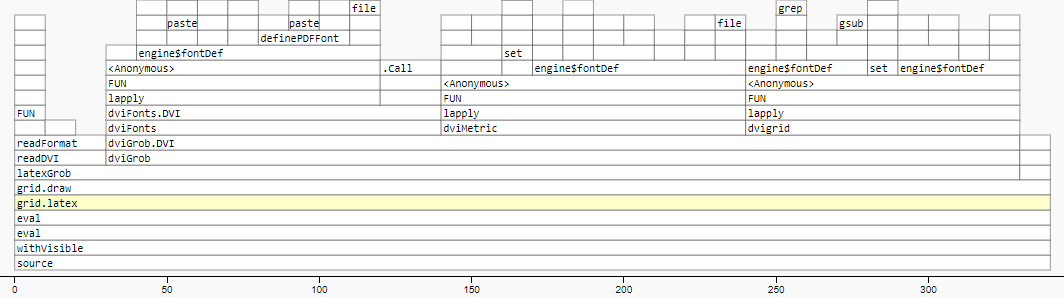
\includegraphics[width=1.00000\textwidth]{../Figures/profilingSimpleProfvis_0.2-1.PNG}
\caption{Screenshot of \texttt{profvis::profvis()} output for the code
\texttt{grid.latex("\$x\ -\ \textbackslash{}\textbackslash{}mu\$")} in
\texttt{dvir} version 0.2-1.}
\end{figure}

We can see the function call stack in figure
@ref(fig:profilingSimpleProfvis\_0.2-1). At the bottom is the call to
\texttt{grid.latex()}, which immediately calls \texttt{grid.draw()}
which in turn calls \texttt{latexGrob()}. This calls \texttt{readDVI()}
for about the first 20ms, then \texttt{dviGrob()} for the remaining time
to the end of the original \texttt{grid.latex()} function call, and so
on up the function call stack.

\begin{figure}
\centering
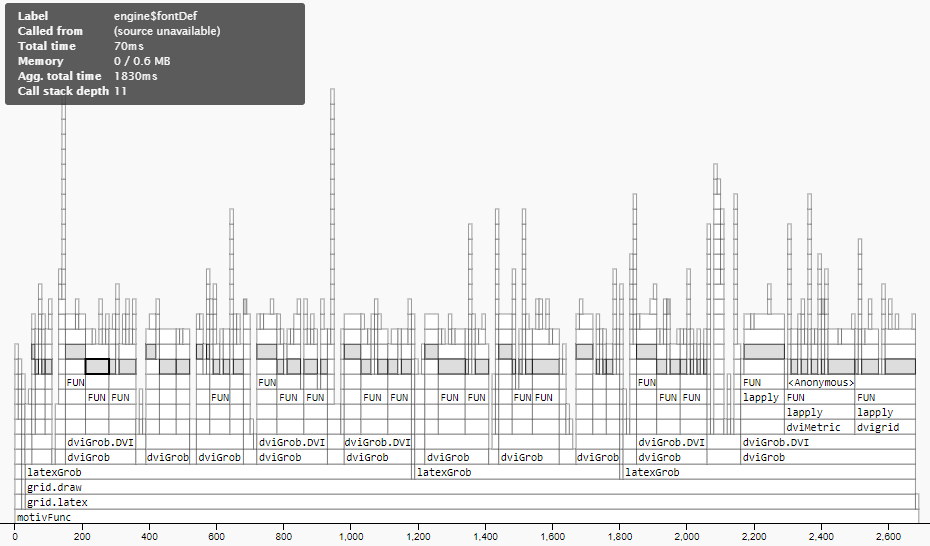
\includegraphics[width=1.00000\textwidth]{../Figures/profilingYeeProfvis_0.2-1_highlight.PNG}
\caption{Screenshot of \texttt{profvis::profvis()} output for the code
creating figure \ref{fig:yeeExample} highlighting the time spent in
\texttt{engine\$fontDef}.}
\end{figure}

The \texttt{profvis::profvis()} output for our more complicated example,
in figure @ref(fig:profilingYeeProfvis\_0.2-1\_highlight) reveals most
of the time to create the figure is in \texttt{grid.latex()}. Note that
the code to draw the arrows and the ``(a)'' in this example is so quick
it occupies the very skinny call stack on the far left of the graph.
\texttt{grid.latex()} and its subsequent function calls, on the other
hand, take up most of the time required to produce the example.

In figure @ref(fig:profilingYeeProfvis\_0.2-1\_highlight) some blocks in
the call stack have been highlighted - these are related to the
\texttt{engine\$fontDef} operation occuring. This is a part of the
``font sweep'', as was described in the introduction to \texttt{dvir} in
section \ref{dvirDesc}.

In the top left corner of figure
@ref(fig:profilingYeeProfvis\_0.2-1\_highlight) we are told the
aggregate time spent with \texttt{engine\$fontDef} is 1830ms. Compared
to the total time of this run (a total of about 2700ms), \texttt{dvir}
is spending a \emph{lot} of time doing these font sweeps.

What was interesting though was that after the actual font sweep the
following sweeps for the metric and grid information \emph{also} called
\texttt{engine\$fontDef}. As the point of the font sweep is that it
finds all the font information to be used later on the following metric
and grid sweeps should not need to ``re-sweep'' for the fonts.

\begin{figure}
\centering
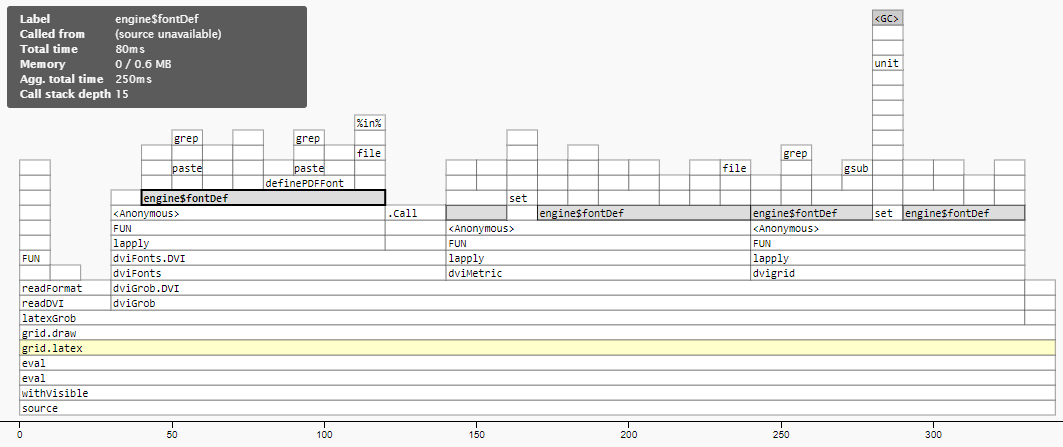
\includegraphics[width=1.00000\textwidth]{../Figures/profilingSimpleProfvis_0.2-1_highlight.PNG}
\caption{Screenshot of \texttt{profvis::profvis()} output for the code
\texttt{grid.latex("\$x\ -\ \textbackslash{}\textbackslash{}mu\$")} in
\texttt{dvir} version 0.2-1, highlighting \texttt{engine\$fontDef}.}
\end{figure}

The effect of this is very obvious in figure
@ref(fig:profilingSimpleProfvis\_0.2-1\_highlight) which is the same as
figure @ref(fig:profilingSimpleProfvis\_0.2-1) but highlights the time
spent in \texttt{engine\$fontDef}. The wrappers for the font, metric and
grid sweeps are \texttt{dviFonts()}, \texttt{dviMetric()} and
\texttt{dvigrid()} respectively (sixth call from the bottom of the
stack). Here we can see nearly all of the time spent in the metric and
grid sweeps are actually redoing the font sweep!

The change to be made was simply stopping the metric and grid sweeps
from doing the font sweep again.

The font sweep looks in the DVI file for op codes 243 to 246. These are
the op codes for font definitions and define the name of a font and give
it an identifier to reference in the DVI file when it wants to use that
font to display a character.

\begin{Shaded}
\begin{Highlighting}[]
\NormalTok{metric_info_}\DecValTok{243}\NormalTok{ <-}\StringTok{ }\NormalTok{op_font_def}
\end{Highlighting}
\end{Shaded}

\begin{Shaded}
\begin{Highlighting}[]
\NormalTok{grid_op_}\DecValTok{243}\NormalTok{ <-}\StringTok{ }\NormalTok{op_font_def}
\end{Highlighting}
\end{Shaded}

Figures @ref\{fig:metricFont\_0.2-1\} and @ref\{fig:gridFont\_0.2-1\}
show the code in the \texttt{dvir} package itself where the metric and
grid sweeps also redid the font sweep. \texttt{op\_font\_def} is a
function which takes the font definition in the DVI file related to that
instance of the op code and searches for and records the font
information.

\begin{Shaded}
\begin{Highlighting}[]
\NormalTok{metric_info_}\DecValTok{243}\NormalTok{ <-}\StringTok{ }\NormalTok{op_ignore}
\end{Highlighting}
\end{Shaded}

\begin{Shaded}
\begin{Highlighting}[]
\NormalTok{grid_op_}\DecValTok{243}\NormalTok{ <-}\StringTok{ }\NormalTok{op_ignore}
\end{Highlighting}
\end{Shaded}

Figures @ref\{fig:metricFont\_0.2-2\} and @ref\{fig:gridFont\_0.2-2\}
show the what the code was changed to in \texttt{dvir} version 0.2-2.
\texttt{op\_ignore} is an empty function, so when the metric or grid
sweeps comes across that op code, they now do nothing.

Unfortunately these changes by themself caused an error when running
\texttt{grid.latex()}. This is because one task undertaken before the
font sweep is to reset or overwrite the global fonts list (which the
font sweep then writes to). The metric and grid sweeps were also doing
this even though it was only intended for it to be done by the font
sweep. This meant after the font sweep was completed it was overwritten
by the metric and grid sweeps and so when \texttt{dvir} tried to draw
the characters there was no font information to refer to.

The resetting of the global fonts list was initiated when the sweeps
passed op code 247 in the DVI file, which is the preamble at the start
of every DVI file.

\begin{Shaded}
\begin{Highlighting}[]
\NormalTok{metric_info_}\DecValTok{247}\NormalTok{ <-}\StringTok{ }\NormalTok{op_ignore}
\end{Highlighting}
\end{Shaded}

\begin{Shaded}
\begin{Highlighting}[]
\NormalTok{grid_op_}\DecValTok{247}\NormalTok{ <-}\StringTok{ }\NormalTok{op_ignore}
\end{Highlighting}
\end{Shaded}

Setting the metric and grid sweeps to do nothing when they pass the
preamble of the DVI file, again by way of \texttt{op\_ignore}, solved
this problem as the global fonts list created by the font sweep is now
not overwritten.

To quantify the impact this has on code speed we recorded the time to
run our examples 20 times, after an initial run to compile the package
after it was loaded.

The second table contains the change in time as a proportion of the
``before'' time.

\begin{figure}

{\centering \includegraphics[width=0.7\linewidth]{Alexander-van-der-Voorn_dissertation_files/figure-latex/speedUp1Simple-1} 

}

\caption{The total time spent in the `grid.latex()` function, metric sweep and grid sweep before and after these changes, over 20 runs of our simple example.}\label{fig:speedUp1Simple}
\end{figure}

For the simple example the time spent in the metric and grid sweeps have
decreased by 76\% and 83\% respectively. The only speed that matters for
users is the overall speed of the call to \texttt{grid.latex()}, which
in this case has decreased by 30\%.

\begin{figure}

{\centering \includegraphics[width=0.7\linewidth]{Alexander-van-der-Voorn_dissertation_files/figure-latex/speedUp1Yee-1} 

}

\caption{The total time spent in the `grid.latex()` function, metric sweep and grid sweep before and after these changes, over 20 runs of our complicated example.}\label{fig:speedUp1Yee}
\end{figure}

Similarly for the more complicated example in figure
@ref\{fig:yeeExample\} the metric and grid sweeps have decreased by 83\%
and 89\% respectively, with \texttt{grid.latex()} overall taking 47\%
less time.

\newpage{}

\section{Code speed (part 2) - font
caching}\label{code-speed-part-2---font-caching}

The earlier code speed up was done by stopping \texttt{dvir} doing
something ``silly''. Our further profiling lead us to find where next
our code spends its time and now it was a matter of making \texttt{dvir}
``smarter''.

- {[}\textbf{Example:} \texttt{profvis()} result showing
\texttt{fontEnc()} (I think) taking long time{]}

\begin{itemize}
\item
  Looks like if we could save/cache a font we could reduce the amount of
  time to run \texttt{grid.latex()}
\item
  \texttt{fonts} R list is re-initialised after every call to
  \texttt{grid.latex()}
\item
  Is a font definition in DVI the same over different calls to
  \texttt{grid.latex()}? Yes! even the font def number (a number
  seemingly determined by TeX)
\end{itemize}

- {[}\textbf{Example:} font definitions from DVI file (over multiple
\texttt{grid.latex()} calls) showing same fonts have same def{]}

\begin{itemize}
\item
  first of all we want the \texttt{fonts} R list to persist over
  multiple \texttt{grid.latex()} calls in an R session. We did this by
  storing fonts list in the \texttt{dvir} environment (using
  \texttt{dvir::set()} and \texttt{dvir::get()})
\item
  When come across a font definition (during a font sweep), we check if
  that font exists - the position in \texttt{fonts} list is determined
  by the font def number, and so as the same fonts (theoretically) have
  the same font def number, we can compare the new font we've come
  across with what is existing in that position in the \texttt{fonts}
  list. If nothing exists in that position in the list, then we save it
  as normal. If a font does exist, then we need to check if it's the
  same (just in case the font def number is not unique for different
  fonts across different \texttt{grid.latex()} calls)
\item
  To do this easiest way was to expand the stored information about
  fonts in \texttt{fonts} to include the hex code chunk (from DVI) of
  the font definition
\item
  Then we check if all parts of the new hex code chunk are the same as
  the existing
\item
  {[}\textbf{Example:} code for new function for checking if two font
  definitions are the same{]}
\item
  If the definitions are the same, do nothing. If they are different,
  overwrite the existing font info with the new font info. This actually
  removes any concern about using only the font def number (which we're
  pretty sure stays the same for the same font, but maybe it doesn't)
\item
  Only requirement is that the font def number is unique within a single
  call to grid.latex() (or rather the resulting DVI output)
\item
  Now only need to change the initialisation (reset) of fonts list to
  happen on package load, rather than during \texttt{grid.latex()} call
  (because doing it every \texttt{grid.latex()} call defeats the purpose
  of storing fonts). Occasionally one might still want to reset the font
  cache, so added an option \texttt{options(dvir.initFonts\ =\ FALSE)}
  and added \texttt{initFonts\ =\ getOption("dvir.initFonts")} to
  \texttt{dviGrob.character()} and \texttt{dviGrob.DVI()}
\item
  {[}\textbf{Example:} show function calls with the above, and anything
  else that helps explain them{]}
\end{itemize}

But why to each of these steps? Need to flesh out more why they achieve
what we want it to achieve (and any considerations we had in our thought
process)

\begin{itemize}
\tightlist
\item
  {[}\textbf{Example:} Profiling results (\texttt{profvis()} and
  \texttt{profmem()} showing speed improvement){]}
\end{itemize}

\subsection{Profiling environment
specifications}\label{profiling-environment-specifications}

The exact results obtained in this and the previous section are specific
to the computing environment used. Specific details are provided below.
The sampling nature of profiling (intermittent recording of the call
stack) will give different results every time it is done.

The profiling results are very specific to the computer setup used and
could change considerably depending on the exact computing environment
in which the \texttt{dvir} package is used.

The profiling results in this report, in this and the next section, were
calculated with the following setup:

\begin{itemize}
\tightlist
\item
  A virtual machine via Oracle VM Virtualbox
\item
  Virtual machine running Ubuntu 18.04.5 LTS
\item
  R version 3.4.4
\item
  \texttt{dvir} package versions as described with the profiling results
\end{itemize}

\newpage{}

\section{Linear gradient fills}\label{linear-gradient-fills}

\subsection{\texorpdfstring{\Tikz{} and
\texttt{dvir}}{ and dvir}}\label{and-dvir}

\Tikz{} is a \TeX{} package that allows drawing of pictures and diagrams
in \TeX{} documents {[}reference \Tikz{} report/description{]}:

\begin{itemize}
\item
  {[}\textbf{Example:} simple \Tikz{} drawing (circles with labels, and
  an arrow maybe){]}
\item
  {[}\textbf{Example:} more complicated \Tikz{} drawing, maybe with
  colouring and stuff{]}
\end{itemize}

The original DVI specification only needed to account for text and
typesetting (and can do the most basic of rectangles too!), and so was
not designed with drawing and graphics in mind. The type of instruction
in the DVI file are labelled with an ``op code''. Each op code described
a type of instruction like defining fonts, setting characters to display
and vertical and horizontal cursor movements. There were four op codes
however, called \emph{DVI specials}, that can contain almost any form of
instruction or values needed, such as text colour, to create a document
based on the DVI file, such as Postscript or PDF.

The \Tikz{} package uses these DVI specials to describe shapes, drawings
and colours in PGF (portable graphics format) which can be translated to
instructions for other viewing formats, like Postscript, PDF or SVG. How
the instructions are translated is controlled by a \Tikz{} driver. The
\texttt{dvir} package includes its own \Tikz{} driver to translate the
drawing instructions into a form useful to draw the things with R grid
graphics {[}reference Paul dvir \Tikz{} report{]}.

Some \Tikz{} features were not implemented though, notably the ability
to have fill colours of shapes as linear or radial gradients or
patterns. The primary reason for this is that R did not support these
types of fills but the latest R release in May 2021, version 4.1.0,
provides support for these fills in the \texttt{grid} package, on which
\texttt{dvir} is built.

\begin{itemize}
\item
  {[}\textbf{Example:} replicate one of the above examples in R{]}
\item
  {[}\textbf{Example:} \Tikz{} radial gradient fill example{]}
\item
  {[}\textbf{Example:} Make same \Tikz{} example as above in R with dvir
  (obviously fill will be blank){]}
\item
  {[}\textbf{Example:} Use R 4.1.0 to make a linear gradient in a
  shape{]}
\end{itemize}

As it is, the \Tikz{} driver simply ignores any gradient or pattern fill
information when creating the DVI file for \texttt{dvir}.

\begin{itemize}
\tightlist
\item
  {[}\textbf{Example:} Use \texttt{grid.tikzpicture()} for picture with
  gradient fill in text, but resulting R graphic does not have fill{]}
\end{itemize}

\subsection{\texorpdfstring{Implementing \Tikz{} linear gradient fills
in
\texttt{dvir}}{Implementing  linear gradient fills in dvir}}\label{implementing-linear-gradient-fills-in-dvir}

The following steps are required to implement these \Tikz{} fills in
\texttt{dvir}:

\begin{enumerate}
\def\labelenumi{\arabic{enumi}.}
\item
  Add the fill information (like the gradient colours and their
  locations) to the DVI file created by \texttt{dvir}
\item
  Store this fill information during a parse by \texttt{dvir} to read
  the DVI file
\item
  Add the fill information when drawing the shape in R
\end{enumerate}

To tackle step 1, we need to update the \texttt{dvir} \Tikz{} driver
file to include information about the gradient and pattern fills. As the
\texttt{dvir} \Tikz{} driver file is based on the SVG \Tikz{} driver
file, the SVG support for \Tikz{} fills was used as a base to edit to
make it specific to \texttt{dvir}.

The information we require for the gradient fills from \Tikz{} via the
DVI file is as per the arguments for the
\texttt{grid::linearGradient(...)}, which is used as an argument to
\texttt{grid::gpar(fill\ =\ linearGradient(...))}, which itself is an
argument to a \texttt{grid} drawing function, for example
\texttt{grid::grid.rect(...,\ gp\ =\ gpar(fill\ =\ linearGradient(...)))}.
The most important parts of defining a linear gradient fill is the
colours and stops of the gradient fill. The stops of a gradient fill are
the locations along the length of a gradient fill where the specified
colours are. In between the stops, the gradient between stop colours
either side occurs.

The \texttt{colours} and \texttt{stops} arguments of
\texttt{linearGradient()} are simply vectors of colours (a character
vector of colour names of hexadecimal RGB values) and locations of those
colours as a proportion of the distance between the start and end points
of the gradient respectively. This obviously guides us as to what
information we need to get from \Tikz{} in the DVI file so we can pass
it to \texttt{dvir}.

Let us consider a simple example, a rectangle with an orange to green
linear gradient fill:

\begin{figure}
\begin{tikzpicture}
\filldraw [draw=black, left color=orange, right color=green] (0,0) rectangle (4,2);
\end{tikzpicture}
\end{figure}

The following is an extract of the DVI file when the rectangle above is
generated using the SVG DVI driver included with the common \TeX{}
distributions, \texttt{pgfsys-dvisvgm.def}. It has been edited slightly
for readability by adding line breaks.

\begin{Shaded}
\begin{Highlighting}[]
\NormalTok{xxx1         k=}\DecValTok{67}
\NormalTok{             x=dvisvgm}\OperatorTok{:}\NormalTok{raw }\OperatorTok{<}\NormalTok{g transform=}\StringTok{"matrix(1,0,0,1,56.90549,28.45274)"}\OperatorTok{>}\NormalTok{\{?nl\} }
\NormalTok{xxx1         k=}\DecValTok{67}
\NormalTok{             x=dvisvgm}\OperatorTok{:}\NormalTok{raw }\OperatorTok{<}\NormalTok{g transform=}\StringTok{"matrix(2.26802,0,0,1.134,0.0,0.0)"}\OperatorTok{>}\NormalTok{\{?nl\} }
\NormalTok{xxx1         k=}\DecValTok{66}
\NormalTok{             x=dvisvgm}\OperatorTok{:}\NormalTok{raw }\OperatorTok{<}\NormalTok{g transform=}\StringTok{"matrix(0.0,1.0,-1.0,0.0,0.0,0.0)"}\OperatorTok{>}\NormalTok{\{?nl\} }
\NormalTok{xxx4         k=}\DecValTok{425}
\NormalTok{             x=dvisvgm}\OperatorTok{:}\NormalTok{raw  }\OperatorTok{<}\NormalTok{linearGradient id=}\StringTok{"pgfsh2"}\NormalTok{ gradientTransform=}\StringTok{"rotate(90)"}\OperatorTok{>}\NormalTok{\{?nl\} }
                            \OperatorTok{<}\NormalTok{stop offset=}\StringTok{" 0.0"}\NormalTok{ stop}\OperatorTok{-}\NormalTok{color=}\StringTok{" rgb(0.0%,100.0%,0.0%) "}\OperatorTok{/}\ErrorTok{>}\NormalTok{\{?nl\} }
                            \OperatorTok{<}\NormalTok{stop offset=}\StringTok{" 0.25"}\NormalTok{ stop}\OperatorTok{-}\NormalTok{color=}\StringTok{" rgb(0.0%,100.0%,0.0%) "}\OperatorTok{/}\ErrorTok{>}\NormalTok{\{?nl\} }
                            \OperatorTok{<}\NormalTok{stop offset=}\StringTok{" 0.5"}\NormalTok{ stop}\OperatorTok{-}\NormalTok{color=}\StringTok{" rgb(50.0%,75.0%,0.0%) "}\OperatorTok{/}\ErrorTok{>}\NormalTok{\{?nl\} }
                            \OperatorTok{<}\NormalTok{stop offset=}\StringTok{" 0.75"}\NormalTok{ stop}\OperatorTok{-}\NormalTok{color=}\StringTok{" rgb(100.0%,50.0%,0.0%) "}\OperatorTok{/}\ErrorTok{>}\NormalTok{\{?nl\} }
                            \OperatorTok{<}\NormalTok{stop offset=}\StringTok{" 1.0"}\NormalTok{ stop}\OperatorTok{-}\NormalTok{color=}\StringTok{" rgb(100.0%,50.0%,0.0%) "}\OperatorTok{/}\ErrorTok{>}\NormalTok{\{?nl\} }
                            \OperatorTok{<}\ErrorTok{/}\NormalTok{linearGradient}\OperatorTok{>}\NormalTok{\{?nl\} }
\NormalTok{xxx1         k=}\DecValTok{57}
\NormalTok{             x=dvisvgm}\OperatorTok{:}\NormalTok{raw }\OperatorTok{<}\NormalTok{g transform=}\StringTok{"translate(-50.1875,-50.1875)"}\OperatorTok{>}\StringTok{ }
\NormalTok{xxx1         k=}\DecValTok{97}
\NormalTok{             x=dvisvgm}\OperatorTok{:}\NormalTok{raw }\OperatorTok{<}\NormalTok{rect width=}\StringTok{"100.375"}\NormalTok{ height=}\StringTok{"100.375"} 
\NormalTok{                            style=}\StringTok{"fill:url(#pgfsh2); stroke:none"}\OperatorTok{/}\ErrorTok{>}\NormalTok{\{?nl\} }
\end{Highlighting}
\end{Shaded}

We can see from this that the linear gradient definition with stops and
colours is defined within a
\texttt{\textless{}linearGradient\textgreater{}} element and given an
\texttt{id} attribute. In the \texttt{\textless{}rect\textgreater{}}
element a CSS style definition sets the fill of the rectangle by
referring to the \texttt{id} of the previously defined definition. In
the linear gradient definition there are colours defined as RGB values
and their respective stops so now we need to get the \texttt{dvir}
driver file to extract the same information in a ``R-friendly'' form.
There are several \TeX{} macros that were defined to do this. These are
based on the \texttt{pgfsys-common-svg.def} and
\texttt{pgfsys-dvisgm.def} SVG drivers that come with most \TeX{}
distributions.

A counter is defined, in order to give each gradient definition unqiue
identifier:

\begin{verbatim}
\newcount\pgf@sys@dvir@objectcount
\end{verbatim}

A ``wrapper'' macro of what to do when a gradient fill is requested.
Within this, the definition of the fill is created and outpu to the DVI
file, followed by

\begin{verbatim}
\def\pgfsys@shadinginsidepgfpicture#1{%
  #1%
  \pgfsysprotocol@literal{SHADING BEING DEFINED: ShadDefID = \the\pgf@sys@dvir@objectcount}%
  \pgf@sys@dvir@sh@defs% 
  \pgf@process{\pgf@sys@dvir@pos}%
  \pgf@xa=-.5\pgf@x%
  \pgf@ya=-.5\pgf@y%
  \pgfsysprotocol@literal{<g transform="translate(\pgf@sys@tonumber{\pgf@xa},\pgf@sys@tonumber{\pgf@ya})">}%
  \pgfsysprotocol@literal{SHADING BEING USED: ShadDefID = \the\pgf@sys@dvir@objectcount}
  \pgf@sys@dvir@sh%
}
\end{verbatim}

\begin{verbatim}
\def\pgfsys@vertshading#1#2#3{%
  {%
    \pgf@parsefunc{#3}%
    \global\advance\pgf@sys@dvir@objectcount by1\relax%
    \pgf@sys@dvir@shading@stops%
    \pgf@sys@dvir@shading@stopcolours%
    \expandafter\xdef\csname @pgfshading#1!\endcsname{%
      \def\noexpand\pgf@sys@dvir@sh@defs{\noexpand\pgfsysprotocol@literal{\pgf@sys@dvir@thestops}}%
      \def\noexpand\pgf@sys@dvir@sh{\noexpand\pgfsysprotocol@literal{<rect
        width="\pgf@sys@tonumber{\pgf@y}"
        height="\pgf@sys@tonumber{\pgf@x}"
        style="fill:url(\noexpand\#pgfsh\the\pgf@sys@dvir@objectcount);
          stroke:none"/>\noexpand\pgfsys@dvir@newline}}%
      \def\noexpand\pgf@sys@dvir@pos{\noexpand\pgfpoint{\the\pgf@y}{\the\pgf@x}}%
    }%
  }%
}
\end{verbatim}

\begin{verbatim}
\let\pgf@sys@dvir@thestops=\pgfutil@empty
\def\pgf@sys@dvir@addtostops#1{%
  \edef\pgf@temp{#1}%
  \expandafter\expandafter\expandafter\def
  \expandafter\expandafter\expandafter\pgf@sys@dvir@thestops
  \expandafter\expandafter\expandafter{\expandafter\pgf@sys@dvir@thestops\expandafter\space\pgf@temp}%
}
\end{verbatim}

\begin{verbatim}
\def\pgf@sys@dvir@shading@stops{%
  % Step 1: Compute 1/\pgf@sys@shading@end@pos
  \pgf@x=\pgf@sys@shading@end@pos\relax%
  \c@pgf@counta=\pgf@x\relax%
  \divide\c@pgf@counta by4096\relax%
  % Step 2: Insert stops locations 
  \pgf@sys@dvir@addtostops{stops=(}%
  \expandafter\pgf@sys@dvir@shading@dostoplocations\pgf@sys@shading@ranges%
  % dummy for end:
  {{\pgf@sys@shading@end@pos}{\pgf@sys@shading@end@pos}}%
  \pgf@sys@dvir@addtostops{)}%
}

\def\pgf@sys@dvir@shading@dostoplocations#1{%
  \edef\pgf@test{#1}%
  \ifx\pgf@test\pgfutil@empty%
  \else%
    \expandafter\pgf@sys@dvir@shading@dostoplocation\pgf@test%
    \expandafter\pgf@sys@dvir@shading@dostoplocations
  \fi%
}

\def\pgf@sys@dvir@shading@dostoplocation#1#2#3#4{%
  % #1 start pos
  % #2 end pos
  % #3 start rgb
  % #4 end rgb
  \pgf@x=#1%
  \pgf@x=16\pgf@x%
  \divide\pgf@x by \c@pgf@counta\relax%
  \expandafter\pgf@sys@dvir@addtostops{\pgf@sys@tonumber\pgf@x}%
}
\end{verbatim}

\begin{verbatim}
\def\pgf@sys@dvir@shading@stopcolours{%
  % Step 1: Compute 1/\pgf@sys@shading@end@pos
  \pgf@x=\pgf@sys@shading@end@pos\relax%
  \c@pgf@counta=\pgf@x\relax%
  \divide\c@pgf@counta by4096\relax%
  % Step 2: Insert stops RGB colours
  \pgf@sys@dvir@addtostops{, colours=(}%
  \expandafter\pgf@sys@dvir@shading@dostopcolours\pgf@sys@shading@ranges%
  % dummy for end:
  {{\pgf@sys@shading@end@rgb}{\pgf@sys@shading@end@rgb}{\pgf@sys@shading@end@rgb}}%
  \pgf@sys@dvir@addtostops{)}%
}

\def\pgf@sys@dvir@shading@dostopcolours#1{%
  \edef\pgf@test{#1}%
  \ifx\pgf@test\pgfutil@empty%
  \else%
    \expandafter\pgf@sys@dvir@shading@dostopcolour\pgf@test%
    \expandafter\pgf@sys@dvir@shading@dostopcolours%
  \fi%
}

\def\pgf@sys@dvir@shading@dostopcolour#1#2#3#4{%
  % #1 start pos
  % #2 end pos
  % #3 start rgb
  % #4 end rgb
  \expandafter\pgf@sys@dvir@shading@dorgb#3%
}
\end{verbatim}

\begin{verbatim}
\def\pgf@sys@dvir@shading@dorgb#1#2#3{%
  \pgf@sys@dvir@color@rgb#1,#2,#3\relax%
  \pgf@sys@dvir@addtostops{\pgf@sys@dvir@prepared}%
}
\end{verbatim}

Section to be continued with:

\begin{itemize}
\item
  What have we had to change in driver file (and why?) - like specific
  bits of driver file.
\item
  Before and after of DVI file (using new driver) for linear gradient
  fill (see new information display). Do the ``after'' for both simple
  rectangle and maybe a more complicated example?
\item
  Why couldn't we go further? Mention the transformations?
\item
  Next steps (to complete steps 1, 2 and 3 as detailed earlier),
  including discussing how this applies to radial gradient fills and
  pattern fills
\end{itemize}

\newpage{}

\section{Text baselines}\label{text-baselines}

\begin{itemize}
\item
  Do all this without examples first maybe, as that will be some fiddly
  work?
\item
  Demonstrate problem (with example using grid.text), especially try
  multi line text maybe?
\item
  Describe algorithms for determining baselines one by one. In dviMoves,
  describe then the issues with choosing which one, and the potential
  algorithms for that
\item
  Describe function I made to calculate all baselines using these
  methods
\item
  Show result of all this (in LaTeX)
\end{itemize}

\subsection{The problem}\label{the-problem}

Text characters have a baseline, that is, a horizontal line on which the
characters naturally sit so all the letters appear to be in line with
each other. Some letters, like a lower case p or j, have a
``descender''. A descender is the part of a character that sits
\emph{below} the baseline. \texttt{grid.text()} accounts for this
baseline so when you bottom align text at a certain y value, the
descenders will actually fall below the y value we defined, despite the
bottom justification. This makes sense because nearly every piece of
written text is like this. Unfortunately, \texttt{grid.latex()} doesn't
account for text baselines. It will simply do any alignment in relation
to bounding box of the text.

To fix this, \texttt{dvir} needs to obtain or calculate a value for the
baseline for any given piece of text to offset the bounding box when it
is drawing text. All of \texttt{dvir}'s information comes from the DVI
file we either need to get a baseline value from the DVI file itself, or
calculate it \emph{from} information in the DVI file. Unfortunately DVI
files do not state a baseline value so we will have to explore some
possible methods to determine a baseline value. These methods are
referred to as algorithms from here on due to their heuristic nature.

\subsection{Implementation}\label{implementation}

To explore the practicality of the algorithms detailed below and
evaluate their usefulness an R function, \texttt{baselines()} has been
created as part of this project. This function takes several arguments,
including the desired baseline selection algorithm, any other
information needed for that particular algorithm, and the \TeX{} code as
you would use with \texttt{grid.latex()}. The output of this function is
the distance, or in some case distances, from the bottom of the bounding
box of the text to the possible baseline value. These distances are
return as \texttt{grid} units.

Now that the potential baselines have been calculated, if when
displaying the text we do not use the specified y value, but rather move
the bounding box down by the amount of the baseline height, it will be
the baseline of the text that is equal to the y-value.

This function has been written to easily allow integration of other
algorithms and most of the function should be able to be directly
implemented in the \texttt{dvir} package, should this baseline algorithm
feature be implemented into \texttt{dvir} formally.

\subsection{Our potential solutions}\label{our-potential-solutions}

We explored several different algorithms to calculate the baseline for
several different types of text that could be used with
\texttt{grid.latex()}. These algorithms are detailed below.

\subsubsection{\texorpdfstring{\texttt{alex}
algorithm}{alex algorithm}}\label{alex-algorithm}

This is a simple algorithm which was determined after inspection of some
DVI files. In every DVI file, there is a statement specifying the size
of the bounding box of the text.

\begin{itemize}
\tightlist
\item
  \textbf{Example} of of the HiResBoundingBox statement here
\end{itemize}

After this statement there appears to consistently be a downward move
the height of the bounding box of text, and then a move upward before
the first character is drawn. This algorithms take the cursor location
after that upward move to be the baseline. In instances where the entire
text has no descenders i.e.~the baseline is the bottom of the bounding
box, there will be no upward move before the first character. In this
case a value of 0 is returned as the baseline.

Here is an example of the \texttt{baselineAlgorithms()} function in
use\ldots{}

\ldots{} and here are some examples showing the text and the calculated
baseline from the function\ldots{}

\begin{Shaded}
\begin{Highlighting}[]
\NormalTok{x <-}\StringTok{ }\NormalTok{grid}\OperatorTok{::}\KeywordTok{unit}\NormalTok{(}\DecValTok{5}\NormalTok{, }\StringTok{"cm"}\NormalTok{)}
\NormalTok{y <-}\StringTok{ "hello"}
\end{Highlighting}
\end{Shaded}

\newsavebox{\dvibox}

\newcommand{\boxreport}[2]{%
  \sbox{\dvibox}{\parbox[b]{1in}{#1}}%
  \usebox{\dvibox}%
  \vspace{-#2}%
  \hrule%
  \vspace{#2}%
}

\boxreport{testing}{0cm}

\boxreport{testing}{0.5mm}

\newcommand\rText{5cm}

\rText

\newcommand\sText{hello}

\sText

\begin{Shaded}
\begin{Highlighting}[]
\KeywordTok{source}\NormalTok{(}\StringTok{"../Appendices/algorithms.R"}\NormalTok{)}
\NormalTok{testText <-}\StringTok{ }\KeywordTok{c}\NormalTok{(}\StringTok{"test"}\NormalTok{,       }\CommentTok{# Text with no danglies}
              \StringTok{"testing"}\NormalTok{,    }\CommentTok{# Text with danglies}
              \StringTok{"var"}\NormalTok{,        }\CommentTok{# Short text with no danglies}
              \StringTok{"varying"}\NormalTok{,    }\CommentTok{# Short text with danglies}
              \StringTok{"$}\CharTok{\textbackslash{}\textbackslash{}}\StringTok{sum_\{n=1\}^\{}\CharTok{\textbackslash{}\textbackslash{}}\StringTok{infty\} 2^\{-n\} = 1$"}\NormalTok{,             }\CommentTok{# Equation only (inline)}
              \StringTok{"$}\CharTok{\textbackslash{}\textbackslash{}}\StringTok{sum}\CharTok{\textbackslash{}\textbackslash{}}\StringTok{limits_\{n=1\}^\{}\CharTok{\textbackslash{}\textbackslash{}}\StringTok{infty\} 2^\{-n\} = 1$"}\NormalTok{,     }\CommentTok{# Equation only (inline, but like 'displaymath')}
              \StringTok{"$}\CharTok{\textbackslash{}\textbackslash{}}\StringTok{sum}\CharTok{\textbackslash{}\textbackslash{}}\StringTok{limits_\{n=1\}^\{\} 2^\{-n\} = 1$"}\NormalTok{,            }\CommentTok{# Equation only (inline, but like 'displaymath' and without upper summation limit)}
              \StringTok{"The equation is $x + }\CharTok{\textbackslash{}\textbackslash{}}\StringTok{frac\{}\CharTok{\textbackslash{}\textbackslash{}}\StringTok{mu^2\}\{2\}$"}\NormalTok{,        }\CommentTok{# Text then equation}
              \StringTok{"The equation is $x + }\CharTok{\textbackslash{}\textbackslash{}}\StringTok{frac\{}\CharTok{\textbackslash{}\textbackslash{}}\StringTok{mu\}\{2\}$"}\NormalTok{,          }\CommentTok{# Text then equation (with lower equation height)}
              \StringTok{"$}\CharTok{\textbackslash{}\textbackslash{}}\StringTok{frac\{}\CharTok{\textbackslash{}\textbackslash{}}\StringTok{mu^2\}\{2\} + x$ is the equation"}\NormalTok{,        }\CommentTok{# Equation then text (with fraction first)}
              \StringTok{"$x + }\CharTok{\textbackslash{}\textbackslash{}}\StringTok{frac\{}\CharTok{\textbackslash{}\textbackslash{}}\StringTok{mu\}\{2\}$ is the equation"}\NormalTok{,          }\CommentTok{# Equation then text (with lower equation height, and fraction first)}
              \StringTok{"}\CharTok{\textbackslash{}\textbackslash{}}\StringTok{begin\{minipage\}\{1in\}Paragraph, with some line wrapping!}\CharTok{\textbackslash{}\textbackslash{}}\StringTok{end\{minipage\}"}\NormalTok{)  }\CommentTok{# Multiline text/paragraph}

\NormalTok{alexAlgorithmBaseline <-}\StringTok{ }\KeywordTok{baselines}\NormalTok{(}\DataTypeTok{tex =}\NormalTok{ testText[}\DecValTok{5}\NormalTok{], }
                                   \DataTypeTok{algorithm =} \StringTok{"alex"}\NormalTok{)}
\NormalTok{alexAlgorithmBaseline}
\end{Highlighting}
\end{Shaded}

\begin{verbatim}
## [1] 688135scaledpts
\end{verbatim}

\subsubsection{\texorpdfstring{\texttt{dviMoves}
algorithm}{dviMoves algorithm}}\label{dvimoves-algorithm}

This is an extension of the \texttt{alex} algorithm. Rather than only
taking the location after the second `down' move, this algorithm keeps
track of \emph{all} the up and down moves of the cursor. The motivation
behind this is that the upward and downward ``moves'' in the DVI file
reflect the cursor moving to the baseline value of the next character to
be typeset. Once again we assume that the first downward move after the
``HiResBoundingBox'' statement id from the top to the bottom of the
bounding box and so this algorithm only returns the upward and downward
cursor moves from there, however as DVI files have the ability to save
the current cursor location, move around a bit, then reset back to the
saved location, all up and down moves are recorded from the start of the
DVI file.

There are two complications with this method:

\begin{itemize}
\item
  As it returns all the vertical positions the cursor moves to there are
  many possible ``baselines'' returned. Any more than one means we have
  to decide which of the baselines values to actually choose
\item
  There are often several up and downward moves in the DVI file between
  typeset characters so in between the ``useful'' baselines there can be
  some which are not so useful or duplicates
\end{itemize}

To account for these considerations, along with the \texttt{dviMoves}
algorithm, the function also allows a choice of method to select a
\emph{single} baseline out of the usually many returned by the
algorithm. These methods are:

\paragraph{\texorpdfstring{\texttt{dviMoves} selection method
\texttt{all}}{dviMoves selection method all}}\label{dvimoves-selection-method-all}

\paragraph{\texorpdfstring{\texttt{dviMoves} selection method
\texttt{index}}{dviMoves selection method index}}\label{dvimoves-selection-method-index}

\paragraph{\texorpdfstring{\texttt{dviMoves} selection method
\texttt{bottomUp}}{dviMoves selection method bottomUp}}\label{dvimoves-selection-method-bottomup}

\paragraph{\texorpdfstring{\texttt{dviMoves} selection method
\texttt{nextChars}}{dviMoves selection method nextChars}}\label{dvimoves-selection-method-nextchars}

\paragraph{\texorpdfstring{Other potential \texttt{dviMoves} selection
methods (not
implemented)}{Other potential dviMoves selection methods (not implemented)}}\label{other-potential-dvimoves-selection-methods-not-implemented}

\begin{itemize}
\item
  best guess
\item
  prev char
\item
  extend dviMoves to only record position just before a character is
  typeset?
\end{itemize}

\subsubsection{\texorpdfstring{\texttt{preview}
algorithm}{preview algorithm}}\label{preview-algorithm}

\subsubsection{\texorpdfstring{\texttt{dvipng}
algorithm}{dvipng algorithm}}\label{dvipng-algorithm}

\subsubsection{any other algorithm?}\label{any-other-algorithm}

\subsection{Discussion of algorithms}\label{discussion-of-algorithms}

Overall, the \texttt{dviMoves} algorithm has performed best out of all
of these. While most of these algorithms perform well for most of the
examples, the \texttt{dviMoves} algorithm performs well for \emph{all}
the examples, notably for giving the option to align the baseline of
\emph{any} line of multi-line text. Utilising the fact it returns all
baseline values for all displayed characters, it is possible to align,
for example, with any character in a mathematical equation, whether it
be of a different size or a superscript or subscript.

\subsection{\texorpdfstring{Next steps to integrate with \texttt{dvir}
package}{Next steps to integrate with dvir package}}\label{next-steps-to-integrate-with-dvir-package}

\begin{itemize}
\item
  mention the ``matching' algorithm of dviMoves (to compare with another
  algorithm)
\item
  mention the ``just ask TeX for answer'' method
\end{itemize}

\newpage{}

\section{Conclusion/summary/next
steps}\label{conclusionsummarynext-steps}

\ldots{} goes here\ldots{}

\end{document}
